\documentclass{article}
\usepackage[utf8]{inputenc}
\usepackage{tikz}

\begin{document}
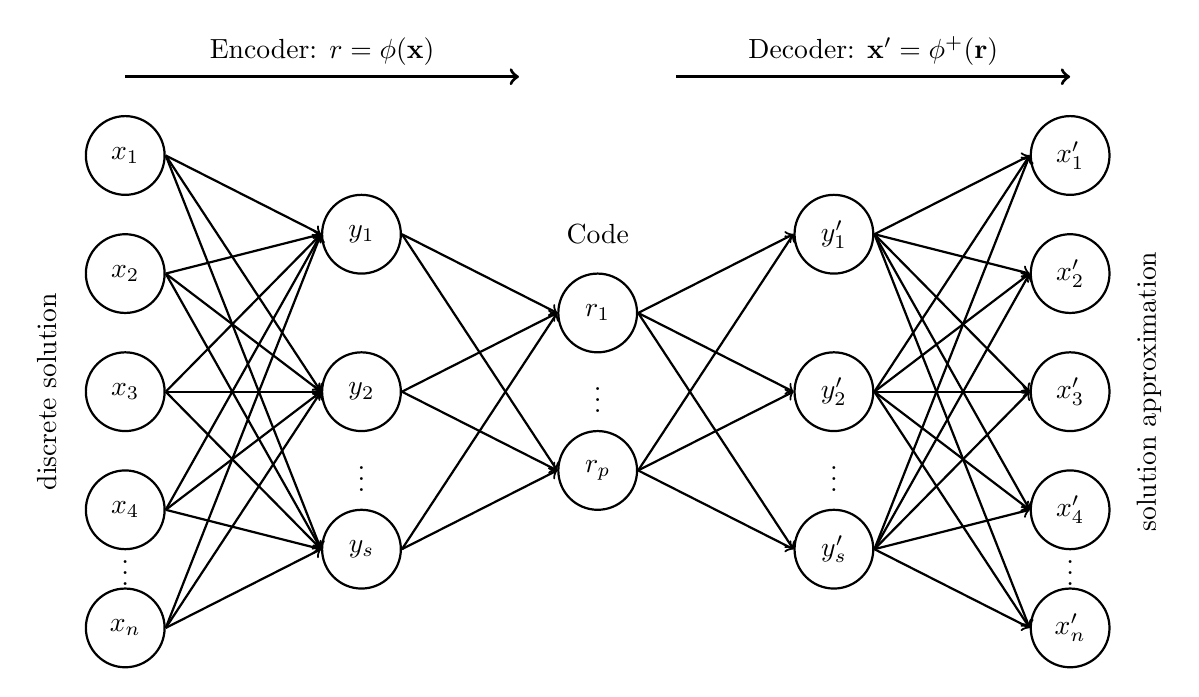
\begin{tikzpicture}
[neuronnode/.style={circle, draw=black, thick, minimum size=10mm},
inputnode/.style={rectangle, draw=black, thick, minimum size=8mm},
connect/.style={->,thick}]
\draw [->, draw=black, very thick] (-4, 4) -- node[above] {Encoder: $r=\phi(\mathbf{x})$} (1, 4);
\draw [->, draw=black, very thick]  (3, 4) -- node[above] {Decoder: $\mathbf{x'}=\phi^+(\mathbf{r})$} (8, 4);
\node [rotate=90] at (-5, 0) { discrete solution};
\node [rotate=90] at (9, 0) {solution approximation};

\node[neuronnode]	(input1) at (-4, 3) {$x_1$};
\node[neuronnode]	(input2) at (-4, 1.5) {$x_2$};
\node[neuronnode]	(input3) at (-4, 0) {$x_3$};
\node[neuronnode]	(input4) at (-4, -1.5) {$x_4$};
\node at (-4, -2.2) {$\vdots$};
\node[neuronnode]	(inputn) at (-4, -3) {$x_n$};
\node[neuronnode]	(neuron1) at (-1, 2) {$y_1$};
\node[neuronnode]	(neuron2) at (-1, 0) {$y_2$};
\node at (-1, -1) {$\vdots$};
\node[neuronnode]	(neuron3) at (-1, -2) {$y_s$};
\node at (2, 2) {Code};
\node[neuronnode]	(neuron4) at (2, 1) {$r_1$};
\node at (2, 0) {$\vdots$};
\node[neuronnode]	(neuron5) at (2, -1) {$r_p$};
\node[neuronnode]	(neuron6) at (5, 2) {$y'_1$};
\node[neuronnode]	(neuron7) at (5, 0) {$y'_2$};
\node at (5, -1) {$\vdots$};
\node[neuronnode]	(neuron8) at (5, -2) {$y'_s$};
\node[neuronnode]	(output1) at (8, 3) {$x'_1$};
\node[neuronnode]	(output2) at (8, 1.5) {$x'_2$};
\node[neuronnode]	(output3) at (8, 0) {$x'_3$};
\node[neuronnode]	(output4) at (8, -1.5) {$x'_4$};
\node at (8, -2.2) {$\vdots$};
\node[neuronnode]	(outputn) at (8, -3) {$x'_n$};
\draw[connect] (input1.east) -- (neuron1.west);
\draw[connect] (input1.east) -- (neuron2.west);
\draw[connect] (input1.east) -- (neuron3.west);
\draw[connect] (input2.east) -- (neuron1.west);
\draw[connect] (input2.east) -- (neuron2.west);
\draw[connect] (input2.east) -- (neuron3.west);
\draw[connect] (input3.east) -- (neuron1.west);
\draw[connect] (input3.east) -- (neuron2.west);
\draw[connect] (input3.east) -- (neuron3.west);
\draw[connect] (input4.east) -- (neuron1.west);
\draw[connect] (input4.east) -- (neuron2.west);
\draw[connect] (input4.east) -- (neuron3.west);
\draw[connect] (inputn.east) -- (neuron1.west);
\draw[connect] (inputn.east) -- (neuron2.west);
\draw[connect] (inputn.east) -- (neuron3.west);
\draw[connect] (neuron1.east) -- (neuron4.west);
\draw[connect] (neuron1.east) -- (neuron5.west);
\draw[connect] (neuron2.east) -- (neuron4.west);
\draw[connect] (neuron2.east) -- (neuron5.west);
\draw[connect] (neuron3.east) -- (neuron4.west);
\draw[connect] (neuron3.east) -- (neuron5.west);
\draw[connect] (neuron4.east) -- (neuron6.west);
\draw[connect] (neuron4.east) -- (neuron7.west);
\draw[connect] (neuron4.east) -- (neuron8.west);
\draw[connect] (neuron5.east) -- (neuron6.west);
\draw[connect] (neuron5.east) -- (neuron7.west);
\draw[connect] (neuron5.east) -- (neuron8.west);
\draw[connect] (neuron6.east) -- (output1.west);
\draw[connect] (neuron6.east) -- (output2.west);
\draw[connect] (neuron6.east) -- (output3.west);
\draw[connect] (neuron6.east) -- (output4.west);
\draw[connect] (neuron6.east) -- (outputn.west);
\draw[connect] (neuron7.east) -- (output1.west);
\draw[connect] (neuron7.east) -- (output2.west);
\draw[connect] (neuron7.east) -- (output3.west);
\draw[connect] (neuron7.east) -- (output4.west);
\draw[connect] (neuron7.east) -- (outputn.west);
\draw[connect] (neuron8.east) -- (output1.west);
\draw[connect] (neuron8.east) -- (output2.west);
\draw[connect] (neuron8.east) -- (output3.west);
\draw[connect] (neuron8.east) -- (output4.west);
\draw[connect] (neuron8.east) -- (outputn.west);

\end{tikzpicture}
\end{document}